\documentclass{beamer}
\usepackage{wrapfig}

\usepackage{graphicx,calc}
\newlength\myheight
\newlength\mydepth
\settototalheight\myheight{Xygp}
\settodepth\mydepth{Xygp}
\setlength\fboxsep{0pt}
\newcommand*\inlinegraphics[1]{%
  \settototalheight\myheight{Xygp}%
  \settodepth\mydepth{Xygp}%
  \raisebox{-\mydepth}{\includegraphics[height=\myheight]{#1}}%
}

\newcommand{\e}{\`E}

\usepackage{booktabs}
\usetheme{Padova}

\title[Gestione \textit{asset} AR]{Gestione \textit{asset} per gemello digitale immerso in realtà aumentata}
\subtitle{Dipartimento di matematica "Tullio Levi-Civita" \\ Corso di laurea triennale in informatica\\ Esame di laurea}
\author{Bellò Marco}
\date{Febbraio 23, 2023}


\begin{document}

	\maketitle

	\begin{frame}{Contenuti}
		\tableofcontents
	\end{frame}

%#######################################################

	\section{Obiettivo}
 
	\begin{frame}{Cos'è un \textit{asset}}
 \begin{figure}[H]
    \centering
    \includegraphics[width=\textwidth]{immagini/cos_e_un_asset.png}
\end{figure}
\centering
\textit{Asset} è gemello digitale di un'entità aziendale \\ \vspace{.5em}
Esempi: stampante, pompa idraulica, telecamera

	\end{frame}
 %#######################################################
	\begin{frame}{Obiettivo}

 \begin{wrapfigure}{l}{0.5\textwidth}
    \centering
    \includegraphics[width=0.245\textwidth]{immagini/asset_card.jpg}\hfill
    \includegraphics[width=0.245\textwidth]{immagini/plant_asset_screenshot.jpg}
\end{wrapfigure}
    

		Realtà aumentata in Flutter\\ \vspace{.5em}
  
Uso di Azure Spatial Anchors \vspace{.5em}

		\begin{itemize}
			\item Comprendere \textit{asset} e realtà aumentata   \vspace{.5em}
			\item Studiare Flutter e linguaggi accessori \vspace{.5em}
			\item Scegliere e integrare \textit{framework} adatto \vspace{.5em}
		\end{itemize}
	\end{frame}
 
%#######################################################

	\section{Tecnologie e strumenti}



%#######################################################

\begin{frame}{Realtà aumentata}

 \begin{wrapfigure}{l}{0.5\textwidth}
    \centering
    \includegraphics[width=0.5\textwidth]{immagini/ancoraggi_multipiano_crop.png}\vspace{.5em}
    \includegraphics[width=0.5\textwidth]{immagini/ikeaAR.jpg}
\end{wrapfigure}
\phantom{A}
\begin{itemize}
    \item Posizionare ancoraggi \vspace{.6em}
    \item Ancoraggi possono essere in relazione tra loro \vspace{.6em}
    \item Agli ancoraggi sono legati oggetti  \vspace{.6em}
    \item Ogni ancoraggio ha una propria \textit{pose} \vspace{.5em}
\end{itemize}
\vspace{3em}
\end{frame}

%#######################################################

\begin{frame}{Framework e Azure Spatial Anchors}

 \begin{wrapfigure}{l}{0.5\textwidth}
    \centering
    \includegraphics[width=0.5\textwidth]{immagini/tecASA.png}\vspace{2em}
    \includegraphics[width=0.5\textwidth]{immagini/aplug_linguaggi.png}
\end{wrapfigure}
Integrazione Flutter e Azure Spatial Anchors (ASA) \vspace{1em}

\begin{itemize}
    \item Azure Spatial Anchors sfrutta gli SDK per l'AR di Android e iOS \vspace{1em}
    \item Il \textit{framework} deve fare da ponte tra ASA e Flutter
\end{itemize}
\vspace{5em}
\end{frame}

%#######################################################

\begin{frame}{Framework realtà aumentata}

 \begin{wrapfigure}{l}{0.5\textwidth}
    \centering
    \includegraphics[width=0.5\textwidth]{immagini/carsius2.png}\vspace{.5em}
    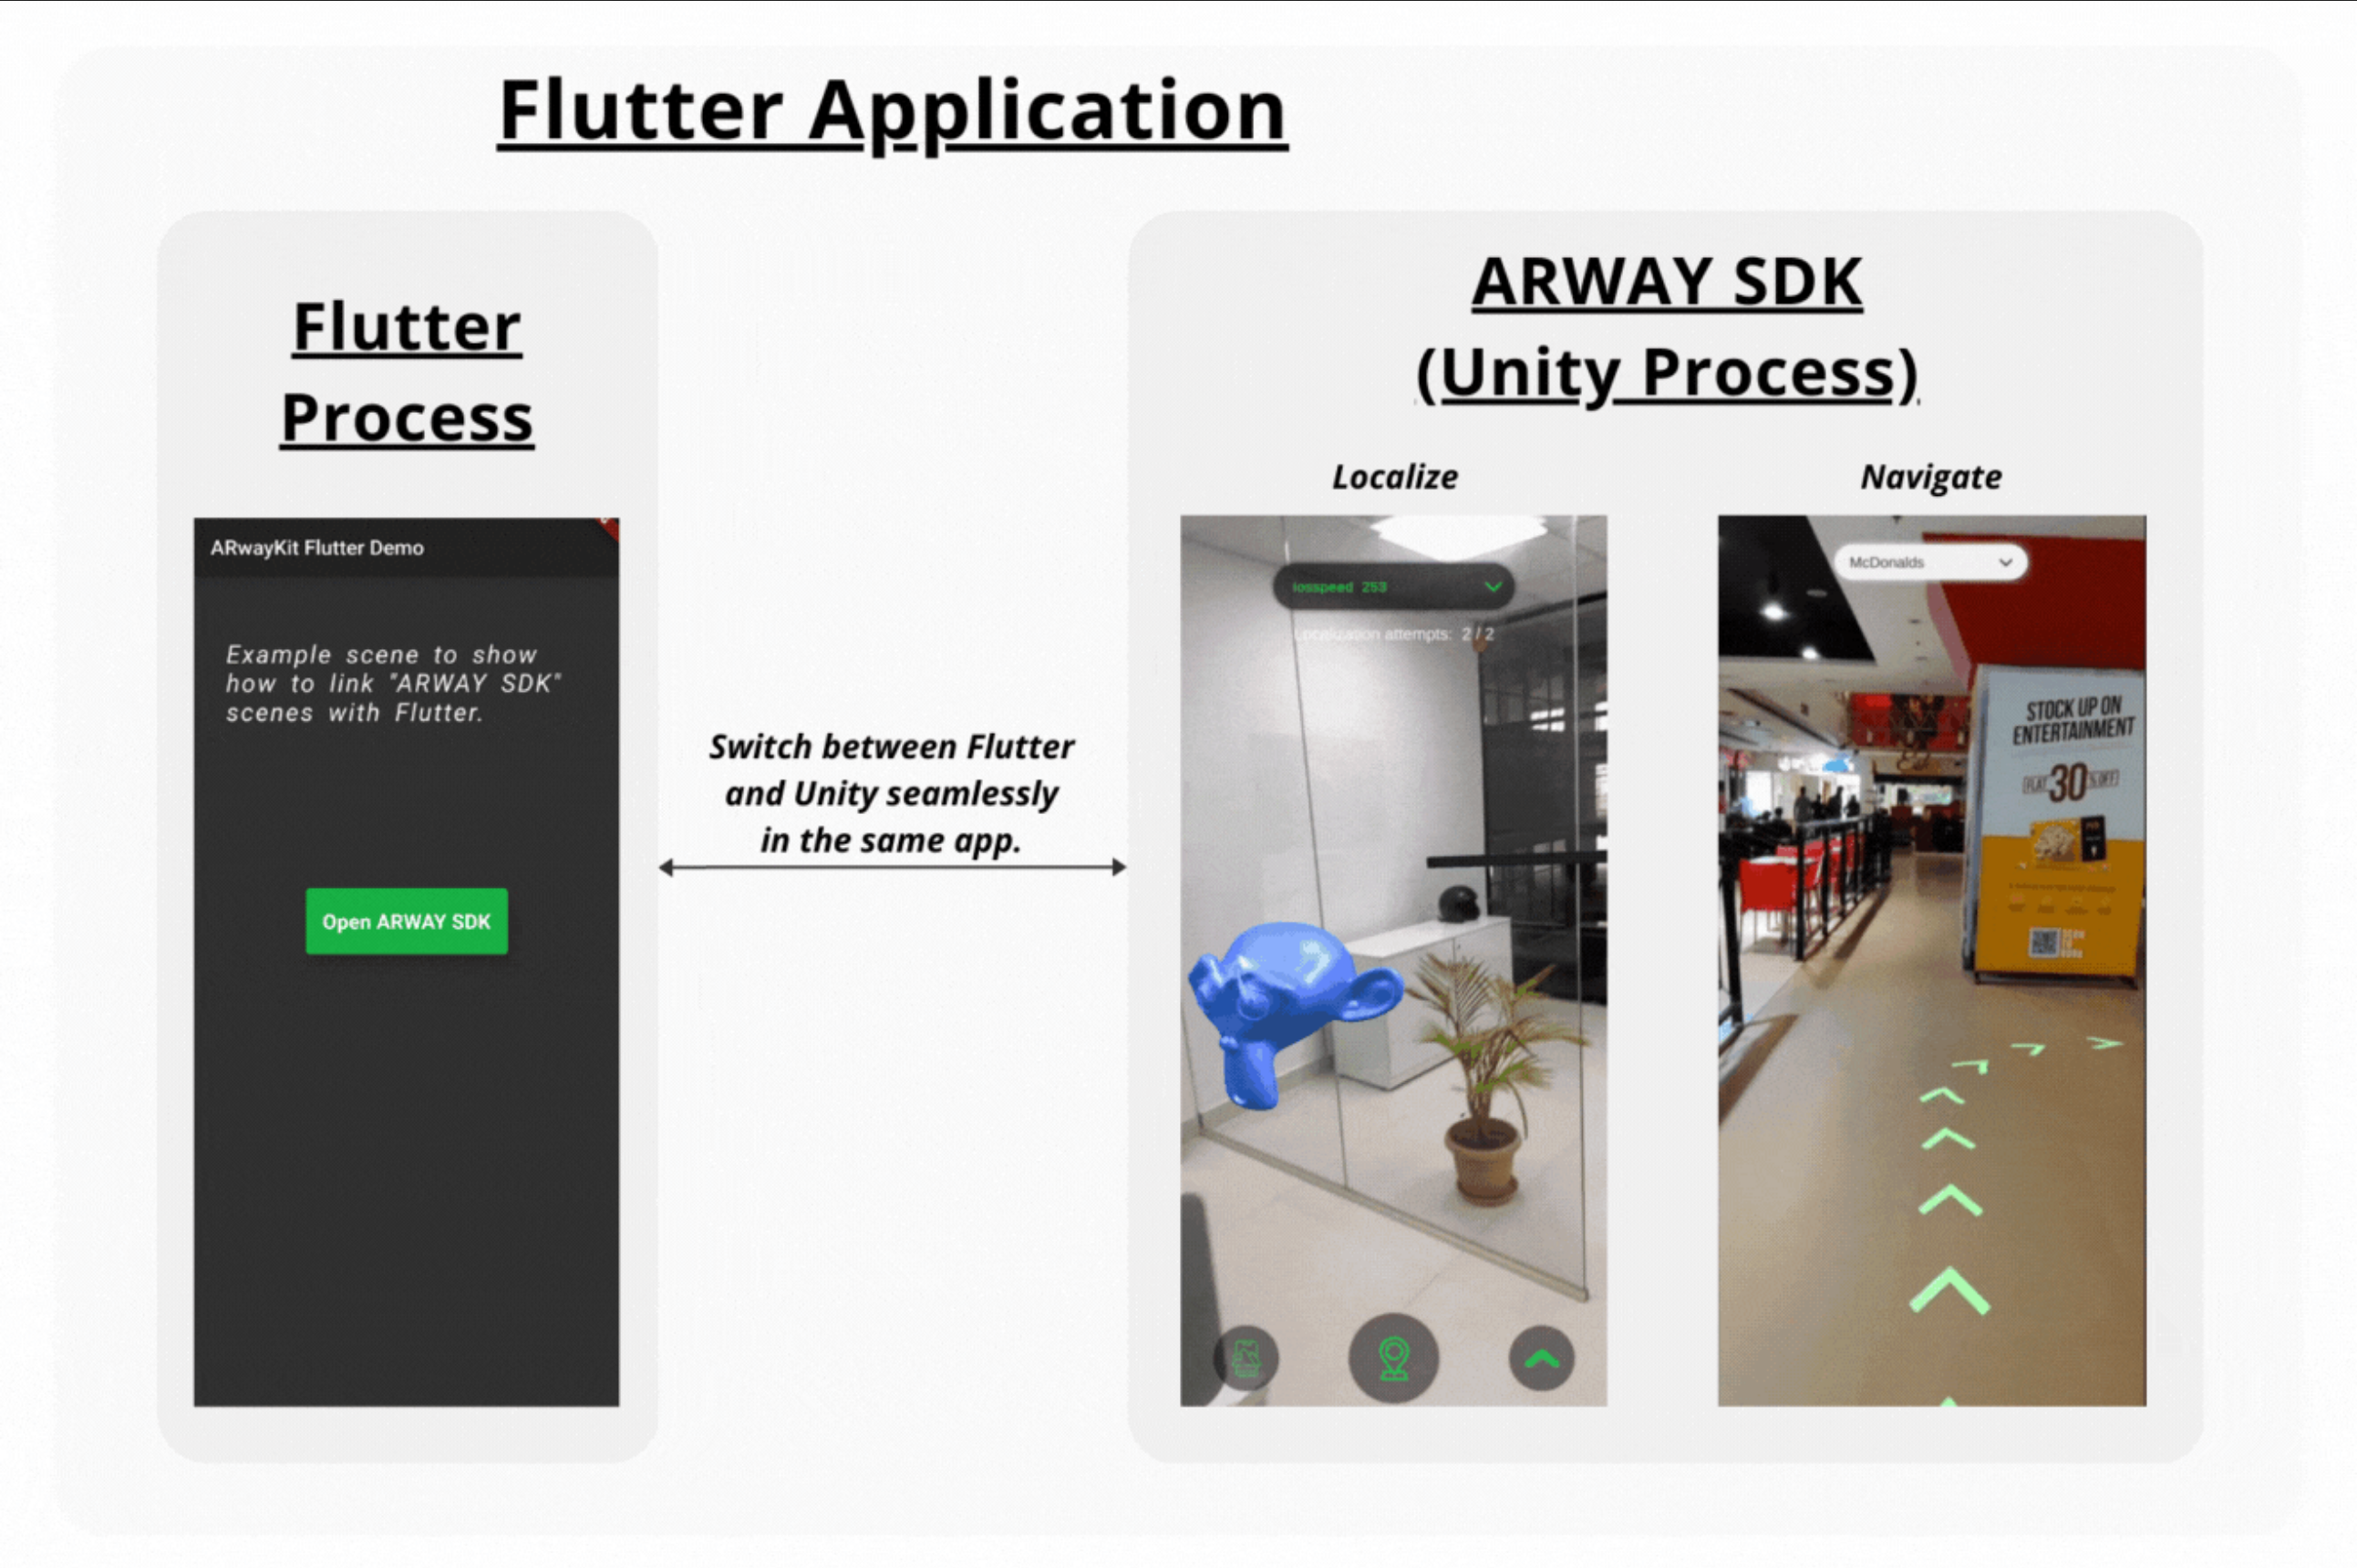
\includegraphics[width=0.5\textwidth]{immagini/ARwayKit_samplegif_screenshot.png}
\end{wrapfigure}

\textbf{ar\_flutter\_plugin}
\begin{itemize}
    \item \inlinegraphics{immagini/freccinaSU.png} Vista AR implementata in Flutter
    \item \inlinegraphics{immagini/freccinaSU.png} Per uso aziendale
    \item \inlinegraphics{immagini/freccinaSU.png} \textit{Open-source}
    \item \inlinegraphics{immagini/freccinaGIU.png} ASA non native
\end{itemize}

\textbf{ARwayKit}
\begin{itemize}
    \item \inlinegraphics{immagini/freccinaSU.png} ASA native 
    \item \inlinegraphics{immagini/freccinaSU.png} Per uso aziendale
    \item \inlinegraphics{immagini/freccinaGIU.png} Vista AR non implementata in Flutter
    \item \inlinegraphics{immagini/freccinaGIU.png} Poca documentazione
\end{itemize}

\vspace{3em}
\end{frame}

%#######################################################

\section{Progettazione}
\begin{frame}{Progettazione architetturale}
 \begin{figure}[H]
    \centering
    \includegraphics[width=\textwidth]{immagini/architettura.png}
\end{figure}
\centering
Architettura del sistema: il \textit{framework} comunica con le ASA\\ \vspace{.5em}
Applicazione cliente ottiene gli identificatori di \textbf{ticket} e \textit{asset} 
\end{frame}

%#######################################################

\section{Risultati}
\begin{frame}{Risultati raggiunti}
 \begin{figure}[H]
    \centering
    \includegraphics[width=0.245\textwidth]{immagini/asset_list.jpg}\hfill
    \includegraphics[width=0.245\textwidth]{immagini/ticket_ar2.jpg}\hfill
    \includegraphics[width=0.245\textwidth]{immagini/asset_card_onTap.jpg}\hfill
    \includegraphics[width=0.245\textwidth]{immagini/remove_asset.jpg}
\end{figure}    
\centering
Lista degli \textit{asset}, \textit{upload} solo se sicuro,
\textit{on-tap} genera \textit{card}

\end{frame}

%#######################################################

\begin{frame}{Difficoltà incontrate}
 \begin{wrapfigure}{l}{0.5\textwidth}
    \centering
    \includegraphics[width=0.5\textwidth]{immagini/asa_flutter_google_search_crop.png}\vspace{0.5em}
    \includegraphics[width=0.5\textwidth]{immagini/asa_flutter_search_today.png}
\end{wrapfigure}
\phantom{a}
\begin{itemize}
    \item Tecnologie nuove \vspace{1em}
    \item Comunicazione tra linguaggi \vspace{1em}
    \item Supporto documentale scarso \vspace{1em}
    \item Poche fonti terze
\end{itemize}
\vspace{4em}
\end{frame}

%#######################################################

\begin{frame}{Impegno orario}
\centering
\small
\begin{table}[h]
\centering
\textbf{Rendicontazione Oraria} \\
\vspace{.5em}
\begin{tabular}{c c c c}
\toprule
\textbf{Obiettivo} & \textbf{Previste} & \textbf{Svolte} & \textbf{Raggiunto} \\
\midrule
Formazione su linguaggi e strumenti &  50 & 60 & Sì\\
\hline
Studio ASA e \textit{framework} & 108 & 100 & Sì \\
\hline
Progettazione & 16 & 30 & Sì\\
\hline
Sviluppo & 116 &130 & 3500 righe\\
\bottomrule
\end{tabular}
\end{table}
  \vspace{0.5cm}
  \centering
  Nel complesso l'esperienza di \textit{stage} è statà positiva\\ \vspace{.5em}
  Arricchente sia da un punto di vista tecnico che professionale
\end{frame}

%#######################################################


\end{document}

\iffalse
		\begin{block}{Normal block}
			Fusce luctus venenatis felis quis semper
		\end{block}

		\begin{alertblock}{Alert block}
			$$ E = (x_1 \vee \neg x_2 \vee \neg x_3) \wedge (x_1 \vee x_2 \vee x_4) $$
		\end{alertblock}

		\begin{exampleblock}{Example block}
			Proin tincidunt, neque at tincidunt mollis
		\end{exampleblock}
\fi